\documentclass{article}

% Language setting
% Replace `english' with e.g. `spanish' to change the document language
\usepackage[english]{babel}

% Set page size and margins
% Replace `letterpaper' with `a4paper' for UK/EU standard size
\usepackage[letterpaper,top=2cm,bottom=2cm,left=3cm,right=3cm,marginparwidth=1.75cm]{geometry}

% Useful packages
\usepackage{amsmath}
\usepackage{graphicx}
\usepackage[colorlinks=true, allcolors=blue]{hyperref}

\title{Example d'Article}
\author{Etienne}
\date{\today}

\begin{document}
\maketitle

\begin{abstract}
Your abstract.
\end{abstract}

\section{Introduction}

Votre introduction va ici! Commencez simplement à rédiger votre document et utilisez le bouton Recompiler pour afficher l'aperçu PDF mis à jour. Des exemples de commandes et de fonctionnalités couramment utilisées sont répertoriés ci-dessous pour vous aider à démarrer.

Une fois que vous êtes familiarisé avec l'éditeur, vous pouvez trouver divers paramètres du projet dans le menu au verso, accessible via le bouton tout en haut à gauche de l'éditeur. Pour consulter des didacticiels, des guides d'utilisation et de la documentation supplémentaire, veuillez visiter notre \href{https://www.overleaf.com/learn}{bibliothèque d'aide}, ou rendez-vous sur notre page de plans vers \href{https://www. overleaf.com/user/subscription/plans}{choisissez votre forfait}.

\section{Quelques exemples pour commencer}

\subsection{Comment créer des sections et des sous-sections}

Utilisez simplement les commandes section et sous-section, comme dans cet exemple de document ! Avec Overleaf, toute la mise en forme et la numérotation sont gérées automatiquement selon le modèle que vous avez choisi. Si vous utilisez l'éditeur visuel, vous pouvez également créer de nouvelles sections et sous-sections via les boutons de la barre d'outils de l'éditeur.

\subsection{Comment inclure des figures}

Vous devez d’abord télécharger le fichier image depuis votre ordinateur en utilisant le lien de téléchargement dans le menu de l’arborescence des fichiers. Utilisez ensuite la commande includegraphics pour l'inclure dans votre document. Utilisez l'environnement figure et la commande caption pour ajouter un numéro et une légende à votre figure. Voir le code de la figure \ref{fig:frog} dans cette section pour un exemple.

Notez que votre figure sera automatiquement placée à l'endroit le plus approprié, compte tenu du texte qui l'entoure et en tenant compte des autres figures ou tableaux qui peuvent se trouver à proximité. Vous pouvez en savoir plus sur l'ajout d'images à vos documents dans cet article d'aide sur \href{https://www.overleaf.com/learn/how-to/Including_images_on_Overleaf}{inclure des images sur Overleaf}.

\begin{figure}
\centering
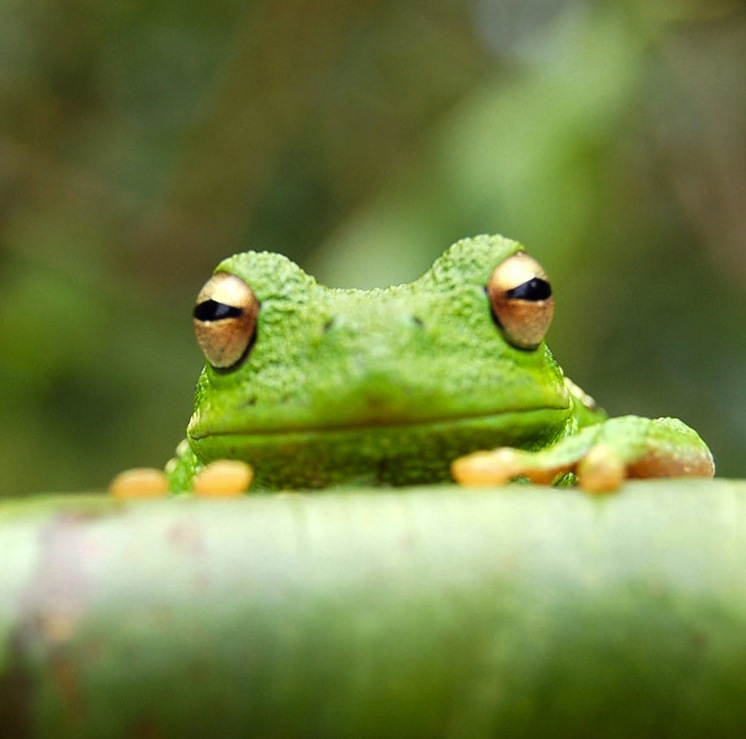
\includegraphics[width=0.25\linewidth]{frog.jpg}
\caption{\label{fig:frog}Cette grenouille a été téléchargée via le menu de l'arborescence des fichiers.}
\end{figure}

\subsection{Comment ajouter des tables}

Utilisez les environnements de table et de tableau pour les tables de base --- voir Table~\ref{tab:widgets}, par exemple. Pour plus d'informations, veuillez consulter cet article d'aide sur \href{https://www.overleaf.com/learn/latex/tables}{tables}.

\begin{table}
\centering
\begin{tabular}{l|r}
Item & Quantity \\\hline
Widgets & 42 \\
Gadgets & 13
\end{tabular}
\caption{\label{tab:widgets}An example table.}
\end{table}

\subsection{Comment ajouter des commentaires et suivre les modifications}

Des commentaires peuvent être ajoutés à votre projet en mettant du texte en surbrillance et en cliquant sur « Ajouter un commentaire » en haut à droite du volet de l'éditeur. Pour afficher les commentaires existants, cliquez sur le menu Révision dans la barre d'outils ci-dessus. Pour répondre à un commentaire, cliquez sur le bouton Répondre dans le coin inférieur droit du commentaire. Vous pouvez fermer le volet Révision en cliquant sur son nom dans la barre d'outils lorsque vous avez terminé la révision pour le moment.

Le suivi des modifications est disponible sur tous nos \href{https://www.overleaf.com/user/subscription/plans}{forfaits premium} et peut être activé ou désactivé à l'aide de l'option en haut du volet Révision. Le suivi des modifications vous permet de suivre chaque modification apportée au document, ainsi que la personne qui effectue la modification.

\subsection{Comment ajouter des listes}

Vous pouvez faire des listes avec numérotation automatique \dots

\begin{enumerate}
\item Comme ça,
\item et comme ça.
\end{enumerate}
\dots ou puces \dots
\begin{itemize}
\item Comme ça,
\item et comme ça.
\end{itemize}

\subsection{Comment écrire les mathématiques}

\LaTeX{} est excellent pour la composition mathématique. Soit $X_1, X_2, \ldots, X_n$ une séquence de variables aléatoires indépendantes et identiquement distribuées avec $\text{E}[X_i] = \mu$ et $\text{Var}[X_i] = \sigma^2 < \infty$, et laissez
\[S_n = \frac{X_1 + X_2 + \cdots + X_n}{n}
       = \frac{1}{n}\sum_{i}^{n} X_i\]
désignent leur moyenne. Ensuite, à mesure que $n$ s'approche de l'infini, les variables aléatoires $\sqrt{n}(S_n - \mu)$ convergent en distribution vers un $\mathcal{N}(0, \sigma^2)$ normal.


\subsection{Comment modifier les marges et le format du papier}

Habituellement, le modèle que vous utilisez aura les marges de page et le format de papier correctement définis pour ce cas d'utilisation. Par exemple, si vous utilisez un modèle d'article de revue fourni par l'éditeur de la revue, ce modèle sera formaté en fonction de ses exigences. Dans ces cas-là, il est préférable de ne pas modifier directement les marges.


Si toutefois vous utilisez un modèle plus général, tel que celui-ci, et que vous souhaitez modifier les marges, une manière courante de le faire consiste à utiliser le package de géométrie. Vous pouvez trouver le package de géométrie chargé dans le préambule en haut de ce fichier d'exemple, et si vous souhaitez en savoir plus sur la façon d'ajuster les paramètres, veuillez consulter cet article d'aide sur \href{https://www.overleaf .com/learn/latex/page_size_and_margins}{taille de la page et marges}.

\subsection{Comment modifier la langue du document et les paramètres de vérification orthographique}

Overleaf prend en charge de nombreuses langues différentes, y compris plusieurs langues différentes au sein d'un même document.

Pour configurer la langue du document, modifiez simplement l'option fournie au package babel dans le préambule en haut de cet exemple de projet. Pour en savoir plus sur les différentes options, veuillez consulter cet article d'aide sur \href{https://www.overleaf.com/learn/latex/International_lingual_support}{support linguistique international}.

Pour modifier la langue de la vérification orthographique, ouvrez simplement le menu au verso en haut à gauche de la fenêtre de l'éditeur, faites défiler jusqu'au paramètre de vérification orthographique et ajustez en conséquence.

\subsection{Comment ajouter des citations et une liste de références}

Vous pouvez simplement télécharger un \verb|.bib| fichier contenant vos entrées BibTeX, créé avec un outil tel que JabRef. Vous pouvez ensuite en citer des entrées, comme ceci : \cite{greenwade93}. N'oubliez pas de spécifier un style de bibliographie, ainsi que le nom du fichier \verb|.bib|. Vous pouvez trouver un \href{https://www.overleaf.com/help/97-how-to-include-a-bibliography-using-bibtex}{tutoriel vidéo ici} pour en savoir plus sur BibTeX.

Si vous disposez d'un \href{https://www.overleaf.com/user/subscription/plans}{compte mis à niveau}, vous pouvez également importer votre bibliothèque Mendeley ou Zotero directement en tant que \verb|.bib| fichier, via le menu de téléchargement dans l'arborescence des fichiers.

\subsection{Bonne chance !}

Nous espérons que Overleaf vous sera utile et jetez un œil à notre \href{https://www.overleaf.com/learn}{help library} pour plus de tutoriels et de guides d'utilisation ! Veuillez également nous faire savoir si vous avez des commentaires en utilisant le lien Contactez-nous au bas du menu au verso --- ou en utilisant le formulaire de contact à l'adresse \url{https://www.overleaf.com/contact}.

\bibliographystyle{alpha}
\bibliography{sample.bib}

\end{document}